\vspace*{-5mm}
\mysection{Specific Requirements}

\mysubsection{Proposed System}
\begin{figure}[H]
	\centering
	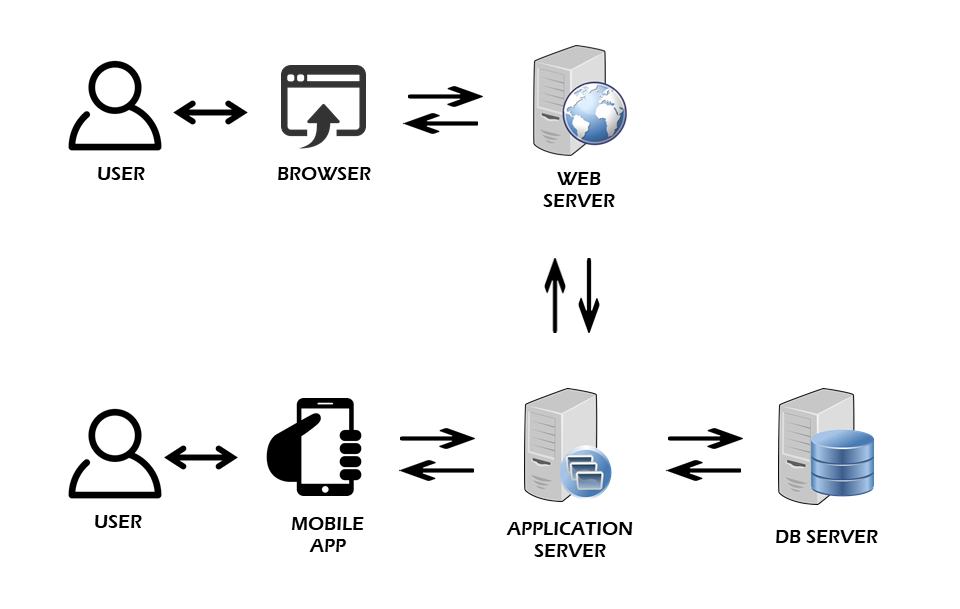
\includegraphics[scale=0.25]{Images/Proposed_System}
	\caption{Proposed System}
\end{figure}

\mysubsection{External Interface Requirements}

\mysubsubsection{User Interfaces}
The following mockups represent an idea of the interfaces that will be provided to the user.
\begin{enumerate}
	\setlength{\leftskip}{1cm}
	\item \textbf{Login}
			\begin{figure}[H]
				\centering
				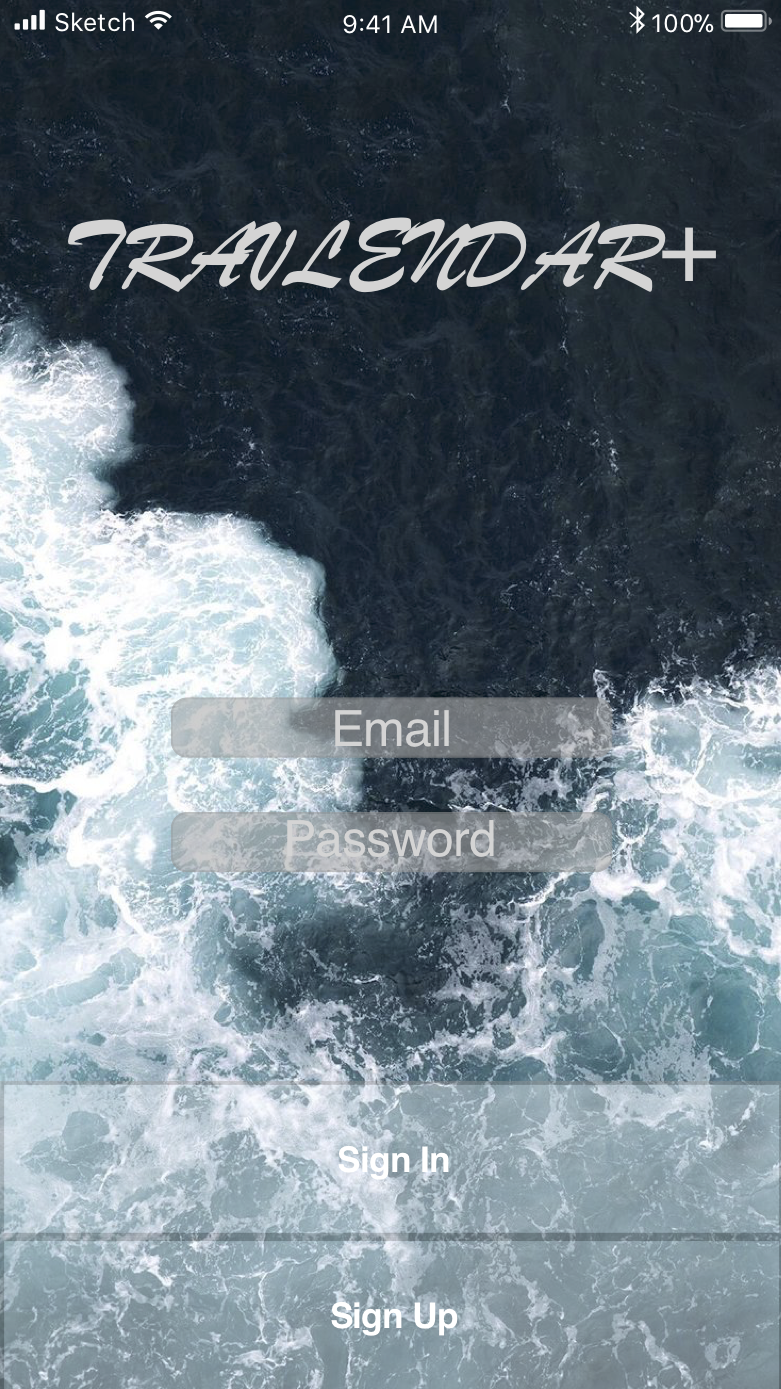
\includegraphics[scale=0.25]{Images/Sketch/Login}
				\caption{Login Sketch}
			\end{figure}
			\newpage
	\item \textbf{User Profile}\\
			\vspace{0cm}\\
			The user will have a personal page in which he will be able to customize his preferences to fit the application to his needs. He will be able to add tags, to edit the lunch section, to select the means of transport he would like the system to use in its computations, and he will also be able to insert his personal season ticket in the homonym field. 
			The system will warn the user with a notification when it is next to the expiry date. 
			\begin{figure}[H]
				\centering
				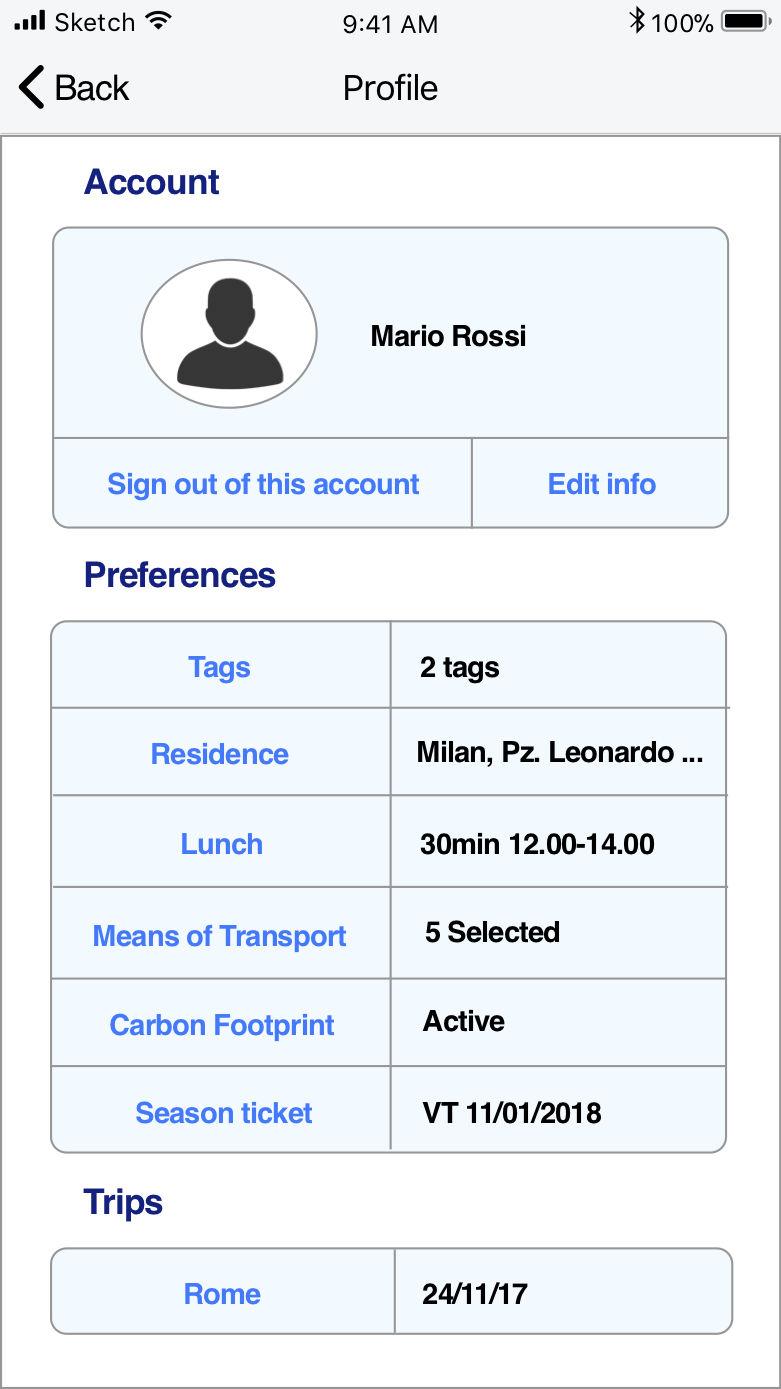
\includegraphics[scale=0.25]{Images/Sketch/User_Profile}
				\caption{User Profile Sketch}
			\end{figure}
	\item \textbf{Event Creation and Trip Planning}\\
			\vspace{0cm}\\
			The user will be able to add an event characterized by a tag icon, which contains the user’s preferences regarding the means of transport and other settings.
			\begin{figure}[H]
				\centering
				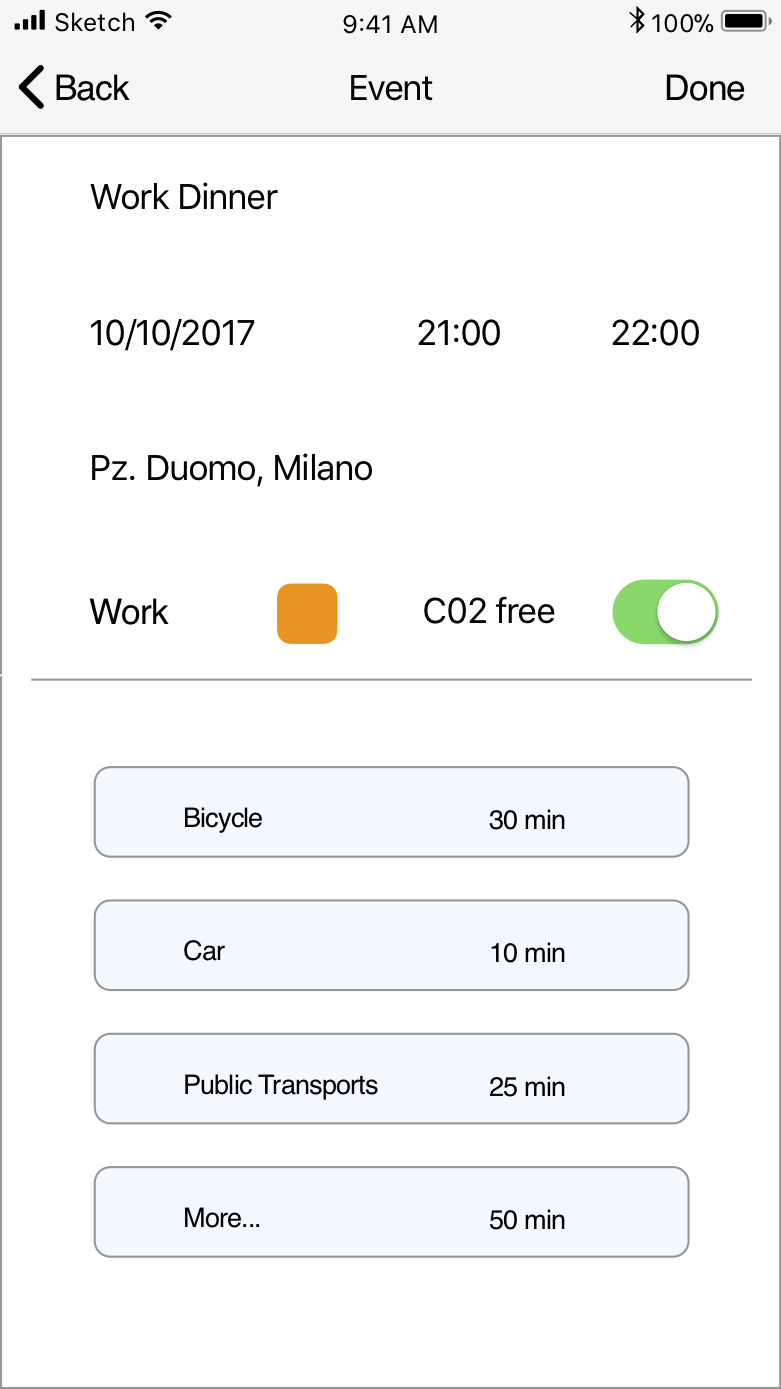
\includegraphics[scale=0.25]{Images/Sketch/Event_Creation_1}
				\hspace{0.5cm}
				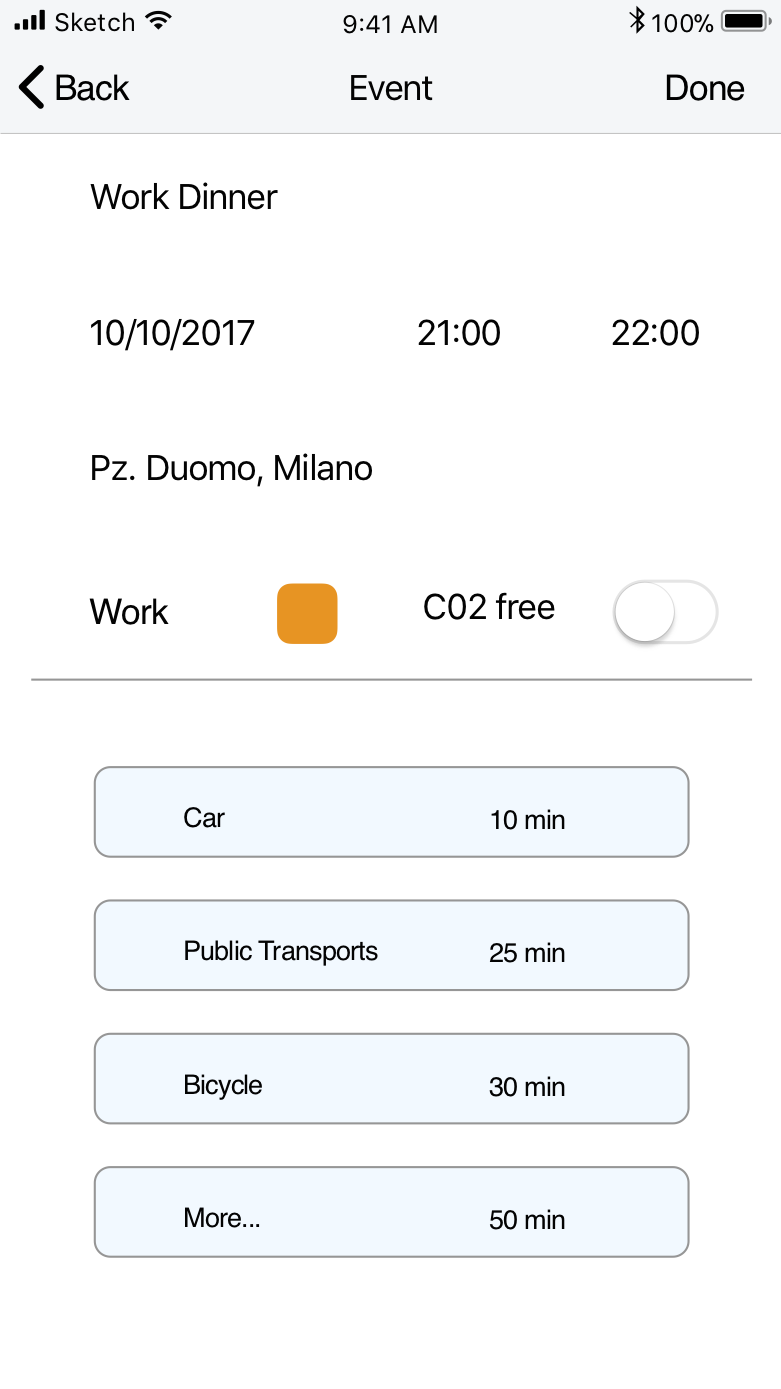
\includegraphics[scale=0.25]{Images/Sketch/Event_Creation_2}
				\hspace{0.5cm}
				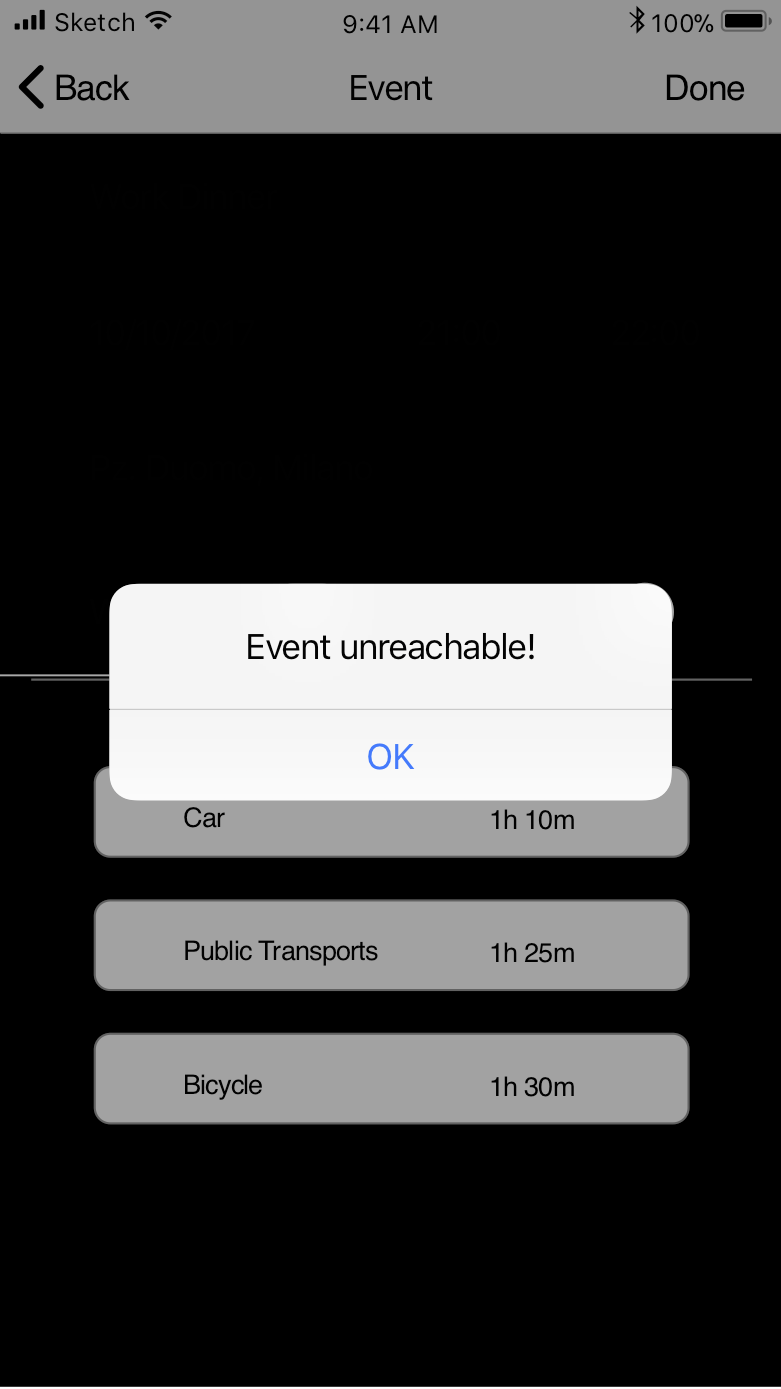
\includegraphics[scale=0.25]{Images/Sketch/Event_Creation_3}
				\caption{Event Creation Sketches}
			\end{figure}
			As shown above the system will suggest the best options to reach the event. If the event is not reachable a warning is displayed.\\
			Otherwise, if the event is not located in the user’s area, the system will suggest the creation of a trip helping the user to book the tickets to reach the desired town.
			\begin{figure}[H]
				\centering
				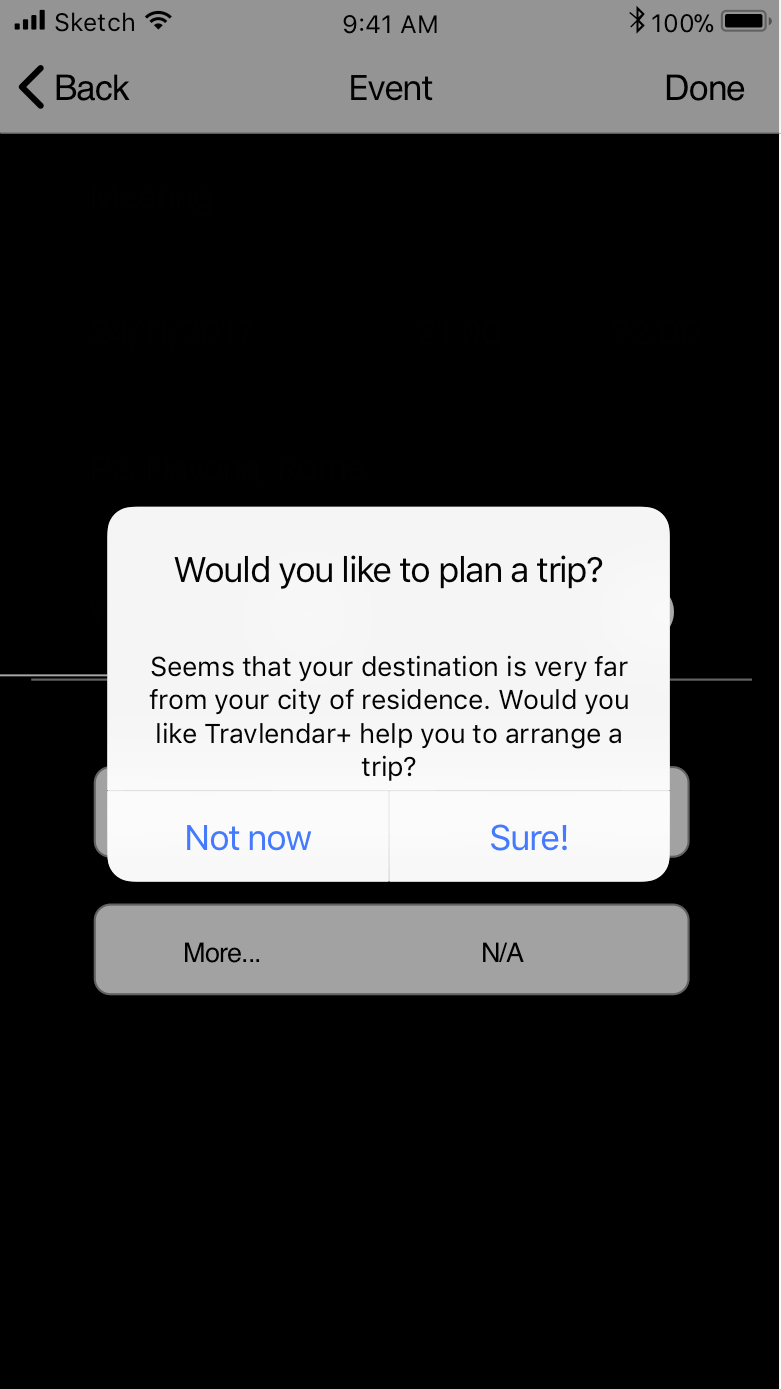
\includegraphics[scale=0.25]{Images/Sketch/Trip_3}
				\hspace{0.5cm}
				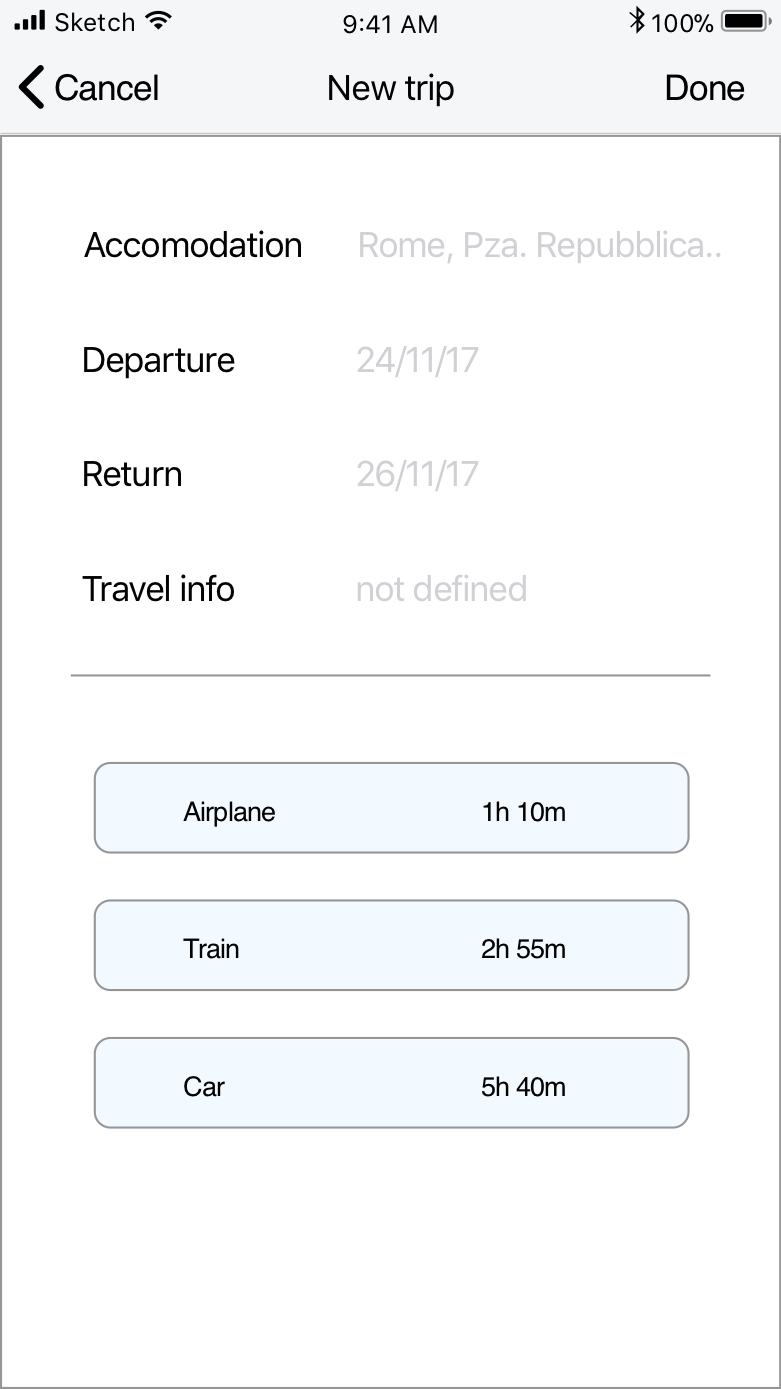
\includegraphics[scale=0.25]{Images/Sketch/Trip_1}
				\hspace{0.5cm}
				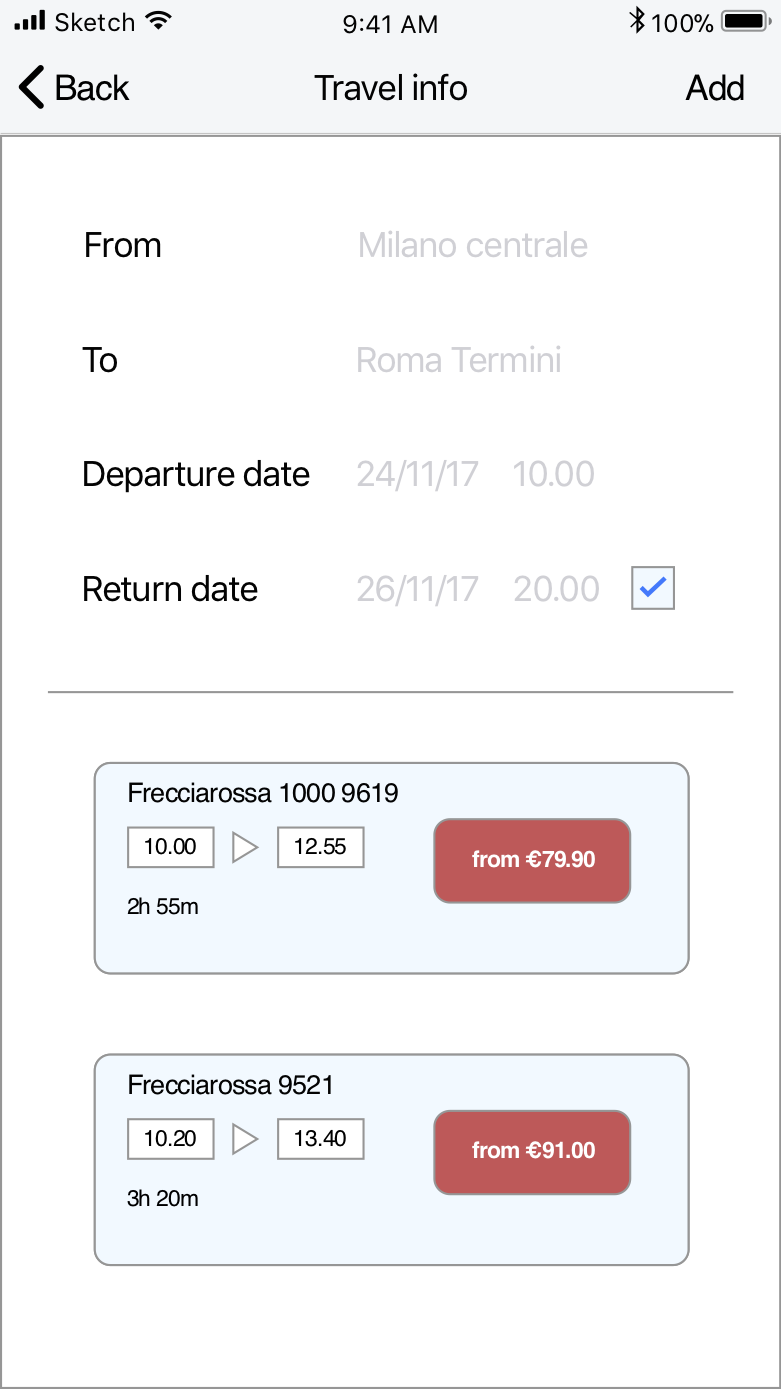
\includegraphics[scale=0.25]{Images/Sketch/Trip_2}
				\caption{Trip Sketches}
			\end{figure}
			If the user wants to plan a trip in advance or in the case he has already planned one, he will be able to add it directly in the Calendar, in the same way he would create an event.
			\begin{figure}[H]
				\centering
				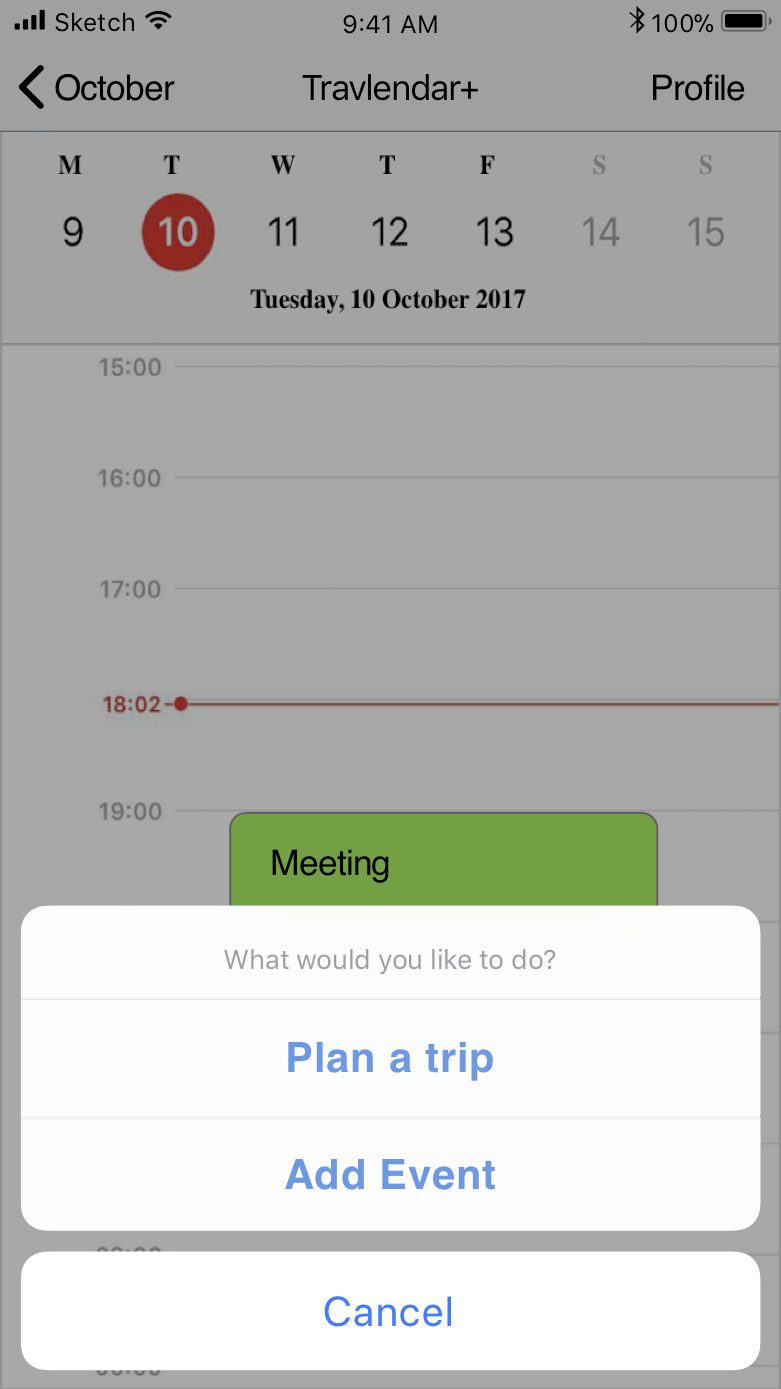
\includegraphics[scale=0.25]{Images/Sketch/Plan_Trip_1}
				\hspace{0.5cm}
				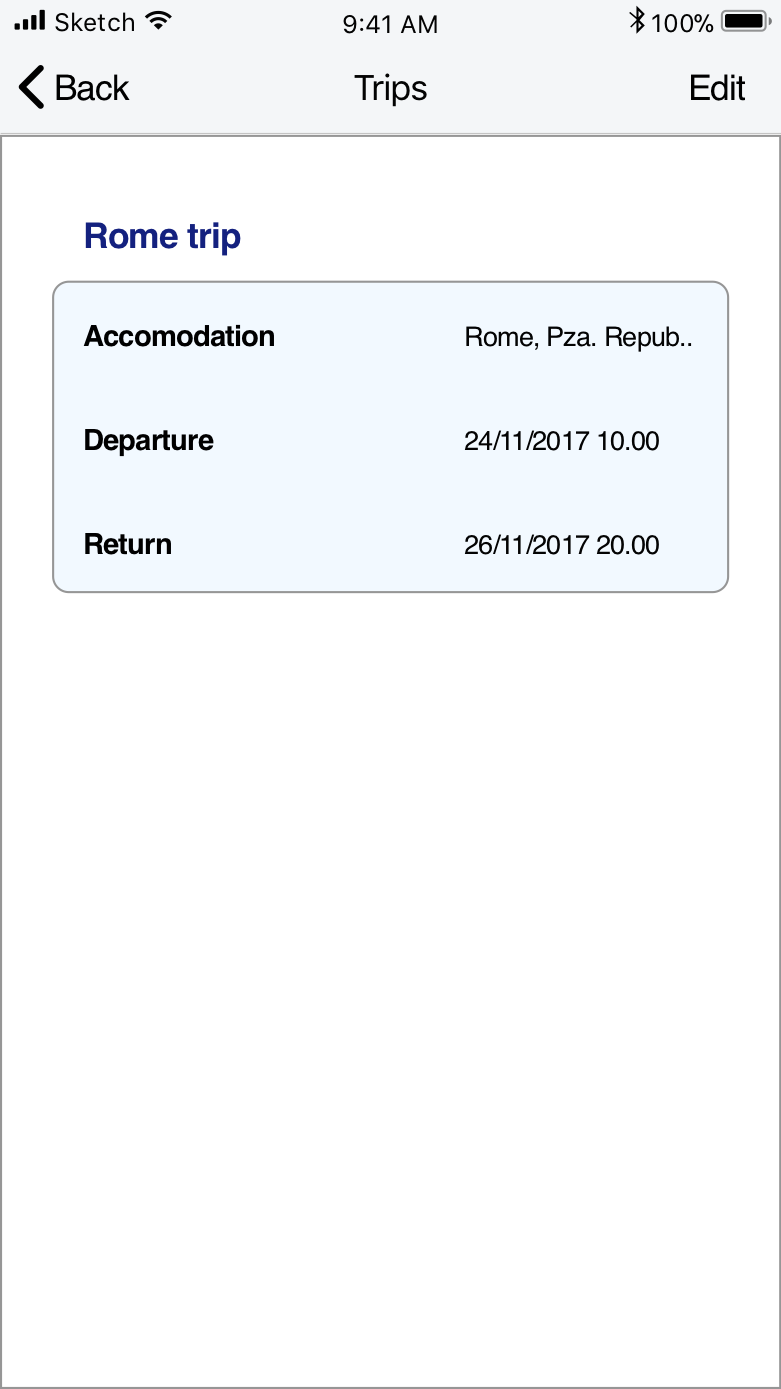
\includegraphics[scale=0.25]{Images/Sketch/Plan_Trip_2}
				\caption{Plan Trip and Trips Sketches}
			\end{figure}
			\newpage
	\item \textbf{Tag Settings}\\
			\vspace{0cm}\\
			In this section the user will be able to create a tag containing a list of the means of transport that can be enabled. It’ll be present another field called “anticipation time” that will be used by the system during the computation of the routes.
			\begin{figure}[H]
				\centering
				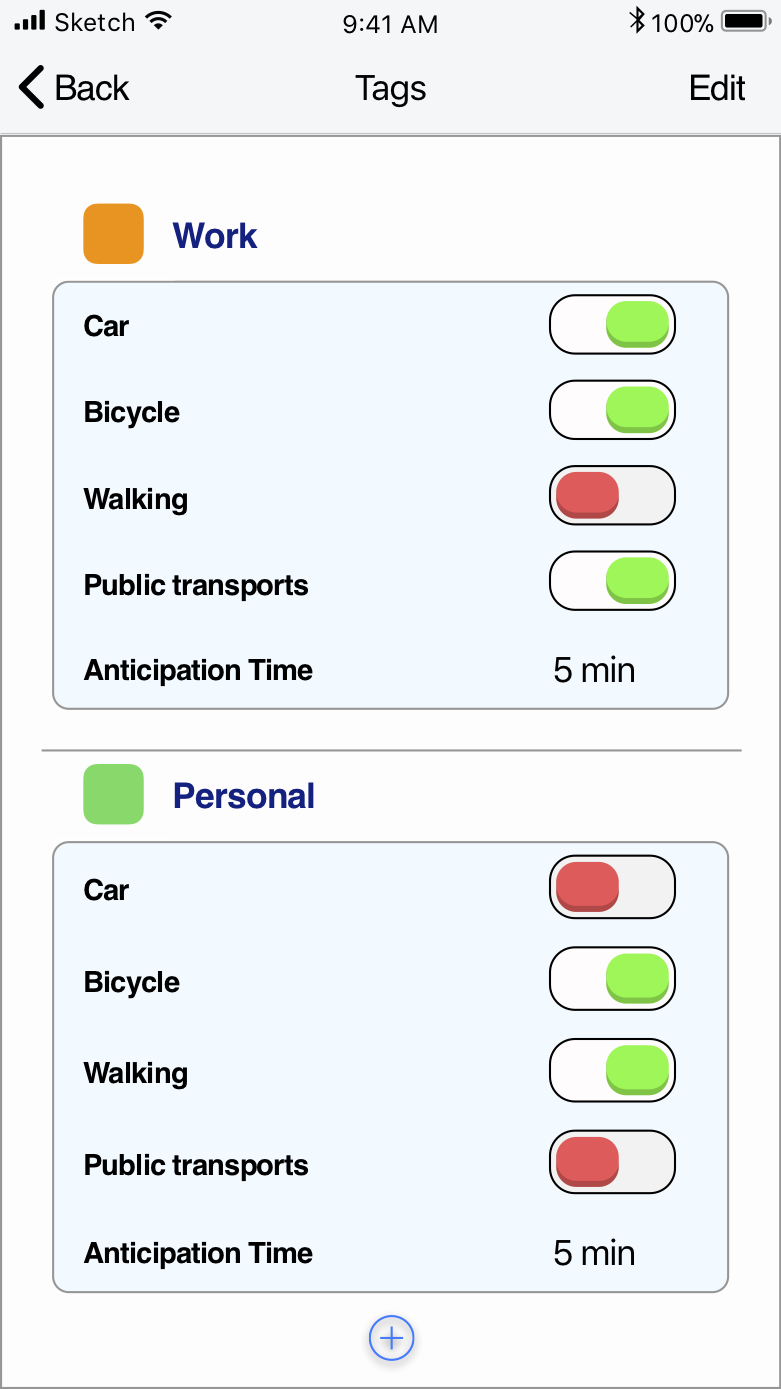
\includegraphics[scale=0.25]{Images/Sketch/Tag}
				\caption{Tag Sketch}
			\end{figure}
	\item \textbf{Event View}\\
			\vspace{0cm}\\
			The user will be able to review his appointments in the calendar section. An arrow will connect each meeting, colored of yellow, in presence of bad weather and strikes, blue when the conditions are optimal.
			\begin{figure}[H]
				\centering
				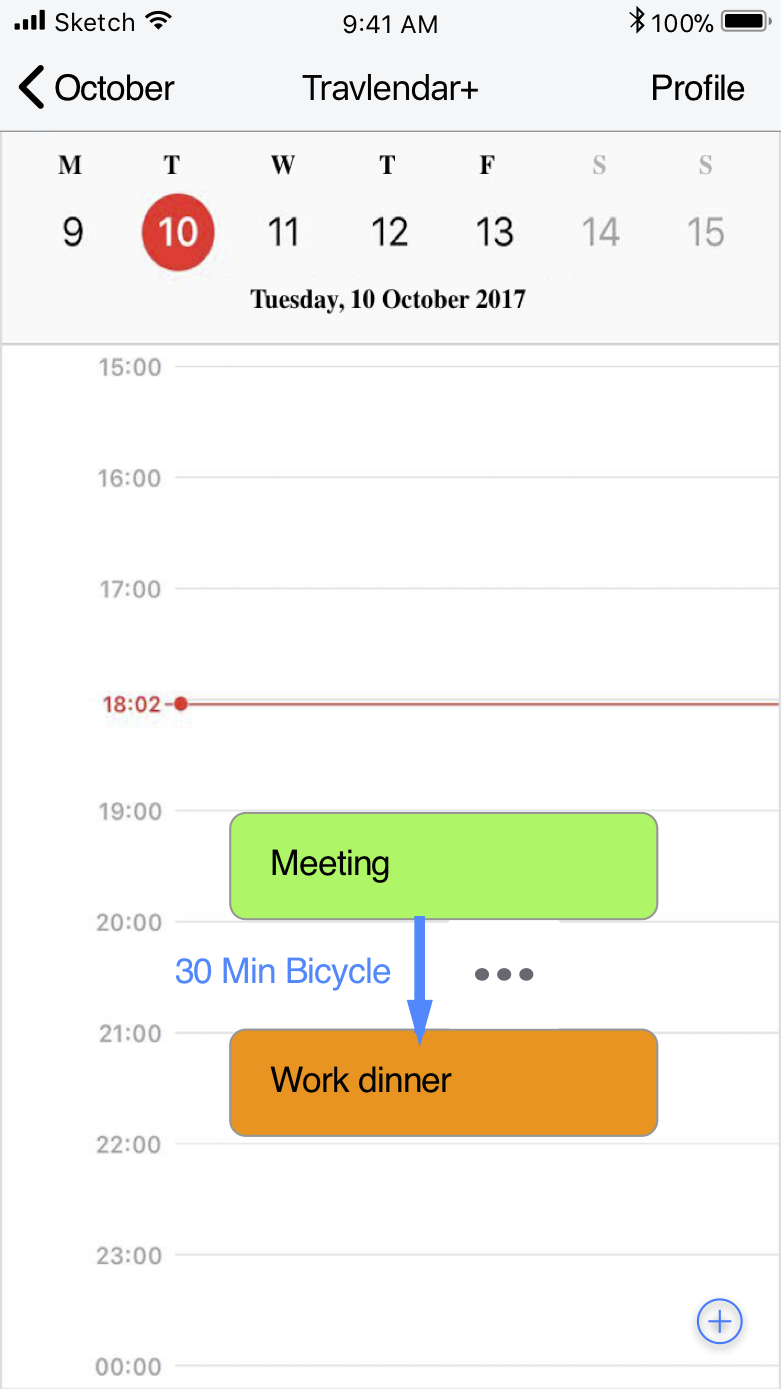
\includegraphics[scale=0.25]{Images/Sketch/Event_View_1}
				\hspace{0.5cm}
				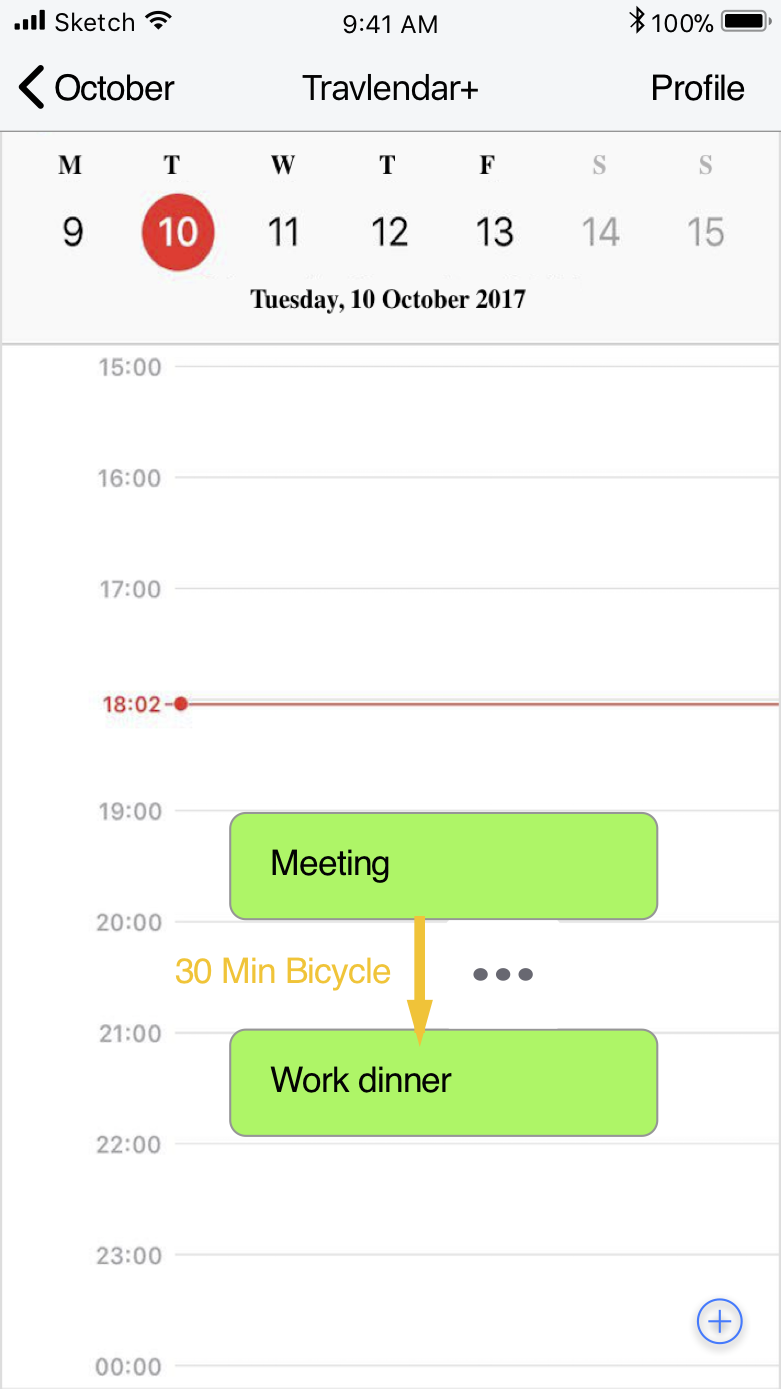
\includegraphics[scale=0.25]{Images/Sketch/Event_View_2}
				\caption{Event View Sketches}
			\end{figure}
			By tapping on the appointment the user will be able to check the directions.
			\newpage
	\item \textbf{Directions}\\
			\vspace{0cm}\\
			\begin{figure}[H]
				\centering
				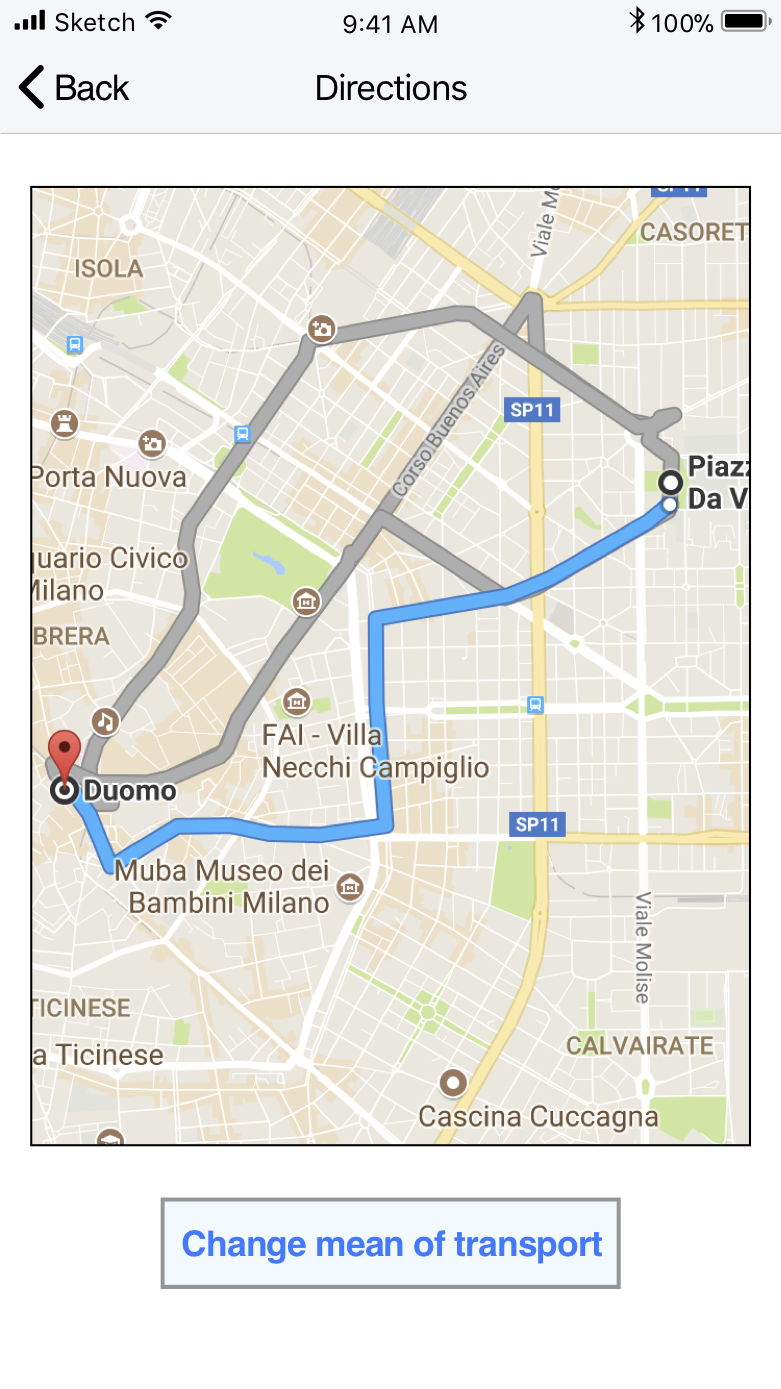
\includegraphics[scale=0.25]{Images/Sketch/Directions}
				\caption{Directions Sketch}
			\end{figure}
\end{enumerate}

\mysubsection{Functional Requirements}
\vspace{0.5cm}
\noindent
\emph{\textbf{[G$_{1}$] : Allow the user to register and log into the system}}
\begin{itemize}
	\setlength{\leftskip}{0.5cm}
	\item \lbrack R$_{1}$] : The System has to check the credentials.
	\item \lbrack R$_{2}$] : A registered user must be able to log in the system.
	\item \lbrack R$_{3}$] : The System has to handle the connection and user requests.
\end{itemize}

\vspace{0.5cm}
\noindent
\emph{\textbf{[G$_{2}$] : Allow the user to add events in the calendar}}
\begin{itemize}
	\setlength{\leftskip}{0.5cm}
	\item \lbrack R$_{1}$] : The system mustn’t allow events overlapping.
	\item \lbrack R$_{2}$] : The system has to guarantee the minimum lunch duration.
	\item \lbrack R$_{3}$] : The system has to give the possibility to the user of arriving on time to the new event.
	\item \lbrack R$_{4}$] : The system has to be able to add the new event to the calendar.
\end{itemize}

\vspace{0.5cm}
\noindent
\emph{\textbf{[G$_{3}$] : Allow the user to receive the mobility options}}
\begin{itemize}
	\setlength{\leftskip}{0.5cm}
	\item \lbrack R$_{1}$] : The system has to check that the event has been created.
	\item \lbrack R$_{2}$] : The system is able to communicate with the route provider.
	\item \lbrack R$_{3}$] : The system sends data about the starting and ending location to the route provider.
	\item \lbrack R$_{4}$] : The system receives the path and the available transports from the route provider.
	\item \lbrack R$_{5}$] : The system has to use the information given in the event’s TAG to filter the possible means of transport.
	\item \lbrack R$_{6}$] : The system has to check the travel means enabled by the user.
	\item \lbrack R$_{7}$] : The system has to obey the constraints set by the user about the travel means.
	\item \lbrack R$_{8}$] : The system has to check if the Carbon footprint preference has been enabled.
	\item \lbrack R$_{9}$] : The system has to retrieve the user's position.
	\item \lbrack R$_{10}$] : The system has to check the weather forecast and strikes.
	\item \lbrack R$_{11}$] : The system has to retrieve the appointment location.
	\item \lbrack R$_{12}$] : The system has to know how to show the solution found.
\end{itemize}

\vspace{0.5cm}
\noindent
\emph{\textbf{[G$_{4}$] : Support the user to avoid getting late on appointment}}
\begin{itemize}
	\setlength{\leftskip}{0.5cm}
	\item \lbrack R$_{1}$] : The system has to retrieve the user's GPS position.
	\item \lbrack R$_{2}$] : The system has to know how to send warnings to the user.
	\item \lbrack R$_{3}$] : The system has to check the destination position.
	\item \lbrack R$_{4}$] : The system has to check the possibility of reaching on time the next event with the slowest mean of transport in the list of suggested ones.
\end{itemize}

\vspace{0.5cm}
\noindent
\emph{\textbf{[G$_{5}$] : Allow the user to have advices about the means of transport that can minimize his carbon footprint}}
\begin{itemize}
	\setlength{\leftskip}{0.5cm}
	\item \lbrack R$_{1}$] : The system must be able to check the carbon footprint preference.
	\item \lbrack R$_{2}$] : The system must know how to filter the means of transport to minimize their carbon footprint.
\end{itemize}

\vspace{0.5cm}
\noindent
\emph{\textbf{[G$_{6}$] : Support the user to have at least 30 minutes of lunch every day}}
\begin{itemize}
	\setlength{\leftskip}{0.5cm}
	\item \lbrack R$_{1}$] : The system must be able to check the lunch preferences.
	\item \lbrack R$_{2}$] : The system must be able to create every day a lunch based on the user's preferences.
	\item \lbrack R$_{3}$] : The system must be able to avoid the creation of those events that prevent the presence of a lunch with the minimum duration.
\end{itemize}

\newpage
\noindent
\emph{\textbf{[G$_{7}$] : Allow the user to buy local transport ticket}}
\begin{itemize}
	\setlength{\leftskip}{0.5cm}
	\item \lbrack R$_{1}$] : The system has to check that all the necessary travel info has been inserted by the user.
	\item \lbrack R$_{2}$] : The system has to address the user to the web site/application to complete the ticket purchase.
\end{itemize}

\vspace{0.5cm}
\noindent
\emph{\textbf{[G$_{8}$] : Give advices about the best transportation ticket to buy}}
\begin{itemize}
	\setlength{\leftskip}{0.5cm}
	\item \lbrack R$_{1}$] : The system has to know how long the user will stay in town.
	\item \lbrack R$_{2}$] : The system has to be able to get information about tickets from the public transport service.
	\item \lbrack R$_{3}$] : The system has to be able to interpret and elaborate the information received.
	\item \lbrack R$_{4}$] : The system has to find the most convenient ticket.
	\item \lbrack R$_{5}$] : The system has to be able to show the results.
\end{itemize}

\vspace{0.5cm}
\noindent
\emph{\textbf{[G$_{9}$] : Remind the user about the expiry date of his season ticket, if he has inserted one}}
\begin{itemize}
	\setlength{\leftskip}{0.5cm}
	\item \lbrack R$_{1}$] : The system has to check the season ticket expiry date.
	\item \lbrack R$_{2}$] : The system has to be able to notify the user that his season ticket is expiring.
\end{itemize}

\vspace{0.5cm}
\noindent
\emph{\textbf{[G$_{10}$] : Allow the user to buy ticket for outdoor travels}}
\begin{itemize}
	\setlength{\leftskip}{0.5cm}
	\item \lbrack R$_{1}$] : The system must check the data inserted by the user to buy the ticket.
	\item \lbrack R$_{2}$] : The system must be able to send the data to the external transport service.
	\item \lbrack R$_{3}$] : The system has to be able to interpret and elaborate the information received.
\end{itemize}

\vspace{0.5cm}
\noindent
\emph{\textbf{[G$_{11}$] : Allow the user to use local sharing services}}
\begin{itemize}
	\setlength{\leftskip}{0.5cm}
	\item \lbrack R$_{1}$] : The system has to retrieve the sharing means location.
	\item \lbrack R$_{2}$] : The system has to check the user's location.
	\item \lbrack R$_{3}$] : The system has to be able to show the sharing mean position to the user.
	\item \lbrack R$_{4}$] : The system has to be able to redirect the user to the external sharing service system for booking the mean.
\end{itemize}

\vspace{0.5cm}
\noindent
\emph{\textbf{[G$_{12}$] : Allow the user to set some preferences in the settings section}}
\begin{itemize}
	\setlength{\leftskip}{0.5cm}
	\item \lbrack R$_{1}$] : The system must be able to show the user the possible preferences.
	\item \lbrack R$_{2}$] : The system has to register these preferences in its database.
	\item \lbrack R$_{3}$] : The system has to have access to these preferences each time is needed.
\end{itemize}

\vspace{0.5cm}
\noindent
\emph{\textbf{[G$_{13}$] : Allow the user to handle his trips}}
\begin{itemize}
	\setlength{\leftskip}{0.5cm}
	\item \lbrack R$_{1}$] : The system has to be able to create travel events.
	\item \lbrack R$_{2}$] : The system has to be able to show the list of trips created.
	\item \lbrack R$_{3}$] : The system has to be able to let the user modify the trips when needed.
	\item \lbrack R$_{4}$] : The system has to be able to check the trips data.
\end{itemize}

\mysubsection{Design Constraints}
\vspace{0.5cm}
\textbf{Regulatory Policies}
\vspace{0.5cm}\par
The system has to ask the users' permission to retrieve and use their positions. Telephone numbers and email addresses won't be used for commercial purposes but just to identify and support the users when needed.
\vspace{0.5cm}\\
\indent \textbf{Hardware Limitations}
\vspace{0.2cm}
\begin{itemize}
	\setlength{\leftskip}{0.5cm}
	\item Mobile App
		\begin{itemize}
			\setlength{\leftskip}{1cm}
			\item iOS or Android Smartphone
			\item 3G/4G Connection
			\item GPS
		\end{itemize}
	\item Web App
		\begin{itemize}
			\setlength{\leftskip}{1cm}
			\item Modern Browser able to retrieve user's location
		\end{itemize}
\end{itemize}

\mysubsection{Non-Functional Requirements}
\vspace{0.5cm}
\textbf{Performance}\par
\vspace{0.2cm}
The system must be able to respond to a large number of user requests simultaneously. The best routes, vehicles and other information, on the application environment, must be provided and calculated as soon as possible and as efficiently as possible.
\newpage

\indent \textbf{Reliability}
\vspace{0.2cm}\par
The system must guarantee a 24/7 service. The information must be stored in a cloud database in order to be always available to the user when required.
\vspace{0.5cm}\\

\indent \textbf{Scalability}
\vspace{0.2cm}\par
Due to the continuous expansion of sharing services and the new way of traveling, the system must ensure a high level of scalability. This skill will also allow Travlendar + to expand by covering more countries and embracing their transport services.
\vspace{0.5cm}\\

\indent \textbf{Security}
\vspace{0.2cm}\par
The data must be encrypted based on the user password and a personal security key. The key must be provided to the user during the account creation. In this way the information will be always available to the user and hidden to those who don’t have the required permissions.
\vspace{0.5cm}\\

\indent \textbf{Accuracy}
\vspace{0.2cm}\par
The information, such as the sharing positions and routes provided by the system, must be as accurate as possible.